\documentclass[11pt,notes=hide,aspectratio=169,mathserif]{beamer}

% PACKAGES
\usepackage{graphics}  % Support for images/figures
\usepackage{graphicx}  % Includes the \resizebox command
\usepackage{url}	   % Includes \urldef and \url commands
\usepackage{natbib}
\usepackage{bibentry}  % Includes the \nobibliography command
\usepackage{verbatim}  %Supports comments
\usepackage{booktabs} %Supports \toprule, \bottomrule, etc in tables
\usepackage{etoolbox}  %Supports toggle commands
\usepackage{datetime}
\usepackage{bm}	%Supports bold math \bm
\usepackage{enumitem}

% TikZ for figures
\usepackage{tikz}
\usetikzlibrary{calc,3d,positioning}

% PACKAGES (that should already be included by your LyX document settings)
\usepackage{amsfonts}  % Lots of stuff, including \mathbb 
\usepackage{amsmath}   % Standard math package
\usepackage{amsthm}    % Includes the comment functions
\usepackage{dsfont}

% CUSTOM DEFINITIONS
\def\newblock{} %Get beamer to cooperate with BibTeX
\linespread{1.2}

\setlist[itemize,1]{label=\usebeamertemplate{itemize item}}
\setlist[itemize,2]{label=\usebeamertemplate{itemize subitem}}
\setlist[itemize,3]{label=\usebeamertemplate{itemize subsubitem}}
\setlist[enumerate,1]{label=\insertenumlabel.}
\setlist[enumerate,2]{label=\insertsubenumlabel.}
\setlist[enumerate,3]{label=\insertsubsubenumlabel.}

% IDENTIFYING INFORMATION
\title[Aldermanic Privilege]{Fragmented Governance, Density, and Housing Affordability:
Evidence from Chicago's Aldermanic Privilege}
\author[Jacob Herbstman]{Jacob Herbstman (University of Chicago)}
\date{\monthname[\the\month] \the\year}

% THEMATIC OPTIONS
\setbeamercovered{transparent}
\usetheme{metropolis}
\usecolortheme{default}
\beamertemplatenavigationsymbolsempty
\setbeamertemplate{footline}[frame number]{}

% BACKUP SLIDE NUMBERING
\usepackage{appendixnumberbeamer}

%SETTINGS
\newtoggle{shortertalk}
\togglefalse{shortertalk}

\begin{document}

%---------------------------------------------------------------------
\begin{frame}[plain]
\titlepage
\note{
	\begin{itemize}
	\end{itemize}
}
\end{frame}
%---------------------------------------------------------------------

% PART 1: MOTIVATION & INSTITUTIONAL SETTING (Slides 2-6)
\section{Motivation}

\begin{frame}
	\begin{itemize}
		\item Chicago alderman have substantial power to shape local land use and development decisions
		\item It has received increased scrutiny in recent years, from both local politicians and the federal government
	\end{itemize}
\end{frame}


\begin{frame}
    \begin{minipage}{0.5\textwidth}
        \begin{figure}
            \centering
            \includegraphics[width=\textwidth]{images/hud_report_headline.png}
			\vspace{20pt}
			\includegraphics[width=\textwidth]{images/lightfoot_order.png}
        \end{figure}
        \end{minipage}
        \hfill
        \begin{minipage}{0.48\textwidth}
        \begin{figure}
            \centering
            \includegraphics[width=\textwidth]{images/old_town_towers.png}
			\vspace{20pt}
			\includegraphics[width=\textwidth]{images/sterling_bay_fight.png}
        \end{figure}
        \end{minipage}
\end{frame}

% PART 2: RELATED LITERATURE (Slide 7)
\begin{frame}
	\begin{itemize}
        \item \textbf{Decentralized Urban Governance}
        \begin{itemize}
            \item {\scriptsize \cite{levine_effects_1999, khan_decentralized_2021,brueckner_bunching_2024, 
            mast_warding_2024,bordeu_commuting_2025}}
        \end{itemize}
        \vspace{1em} 

        \item \textbf{Incumbent Residents' Influence on Development}
        \begin{itemize}
            \item \scriptsize{\cite{fischel_homevoter_2009, rossihansberg_housing_2010, ortalo-magne_political_2014,freemark_upzoning_2020}}
        \end{itemize}
        \vspace{1em}
    
        \item \textbf{Spatial Regression Discontinuity Designs}
        \begin{itemize}
            \item \scriptsize{\cite{black_better_1999,bayer_unified_2007,turner_land_2014,monarrez_dividing_2023}}
        \end{itemize}
        \vspace{1em}
    
    \end{itemize}
\end{frame}


% PART 3: SIMPLE THEORY (Slides 8-9)
% ==============================================================================
% SLIDE 7: TOY MODEL - SETUP
% ==============================================================================
\begin{frame}
	\frametitle{A Toy Model of Aldermanic Behavior}
	\small
	Adapts \cite{bordeu_commuting_2025} framework for infrastructure misallocation
	
	\vspace{0.5em}
	\textbf{Setup:} City divided into $g$ wards; total housing $H = \sum_g h_g$
	
	\vspace{0.5em}
	\begin{itemize}
		\item $A(H)$: \textbf{Citywide benefits} of housing --- tax revenue, affordability, agglomeration
		\begin{itemize}
			\item \textit{Diffuse}: shared across the whole city
			\item $A'(H) > 0$, $A''(H) < 0$
		\end{itemize}
		\vspace{0.3em}
		\item $C(h_g)$: \textbf{Local congestion costs} --- traffic, parking, neighborhood character
		\begin{itemize}
			\item \textit{Concentrated}: borne by ward $g$ where construction occurs
			\item $C'(h) > 0$, $C''(h) > 0$
		\end{itemize}
		\vspace{0.3em}
		\item $\lambda \in (0,1)$: Fraction of citywide benefits the alderman internalizes
	\end{itemize}
\end{frame}


% ==============================================================================
% SLIDE 8: TOY MODEL - UNDERPROVISION AND PREDICTIONS
% ==============================================================================
\begin{frame}
	\frametitle{Under-Provision and Testable Predictions}
	\small
	\textbf{Alderman} maximizes: $V = \lambda A(H) - C(h)$ \quad $\Rightarrow$ FOC: $\lambda A'(H) = C'(h)$
	
	\vspace{0.3em}
	\textbf{Planner} maximizes: $W = A(H) - C(h)$ \quad $\Rightarrow$ FOC: $A'(H) = C'(h)$
	
	\vspace{0.5em}
	Since $\lambda < 1$: \quad $\boxed{h^{\text{decentralized}} < h^{\text{planner}}}$
	
	\vspace{0.3em}
	\textit{Intuition}: Alderman stops building when local costs outweigh \textit{their share} of benefits
	
	\vspace{0.5em}
	\textbf{Comparative statics:}
	\begin{itemize}
		\item $\partial h^* / \partial \lambda > 0$ \quad (more internalization $\rightarrow$ more housing)
	\end{itemize}
	
	\vspace{0.3em}
	\textbf{Testable predictions:}
	\begin{enumerate}
		\item Stricter aldermen (low $\lambda$, as proxied by permit processing times) $\rightarrow$ lower density
		\item Lower density $\rightarrow$ higher rents and home prices
	\end{enumerate}
\end{frame}


% PART 4: MEASURING ALDERMAN STRICTNESS (Slides 10-12)
% ==============================================================================
% SLIDE 9: THE CHALLENGE - MEASURING STRICTNESS
% ==============================================================================
\begin{frame}
	\frametitle{The Challenge: Measuring Alderman Strictness}
	\begin{itemize}
		\item Alderman preferences/frictions are latent: need to infer from observed behavior
		\item \textbf{Idea}: Use permit processing times as a \textbf{proxy} for regulatory strictness
		\begin{itemize}
			\item Data: Universe of Permits in Chicago (2006-2025) from Department of Buildings
			\item Longer average processing time $\rightarrow$ more back-and-forth, more friction 
		\end{itemize}
		\item Focus on \textbf{high-discretion permits}: new construction, renovation, demolition
	\end{itemize}
\end{frame}


% ==============================================================================
% SLIDE 10: STRICTNESS SCORE CONSTRUCTION
% ==============================================================================
\begin{frame}
	\frametitle{Strictness Score Construction}
	\begin{enumerate}
		\item \textbf{Residualize} processing times on ward characteristics + year $\times$ month FEs
		\begin{itemize}
			\item Controls for baseline differences across wards (income, development activity, etc.)
		\end{itemize}
		\item \textbf{Estimate alderman fixed effects} on residualized processing times
		\[
			\widehat{\epsilon}_{it} = \mu + \delta_a + \eta_{it}
		\]
		\vspace{-0.5em}
		\item \textbf{Empirical Bayes shrinkage} to reduce noise {\scriptsize \citep{kline_systemic_2022,kline_discrimination_2024}} then standardize to mean 0, SD 1
	\end{enumerate}
	
	\vspace{0.5em}
	\textbf{Interpretation}: High score = alderman associated with longer processing times
	
	\vspace{0.3em}
	\textbf{Caveat}: This is a \textit{proxy} --- likely understates true variation
	\begin{itemize}
		\item Misses projects that never apply or are discouraged early
	\end{itemize}
\end{frame}


% ==============================================================================
% SLIDE 11: ALDERMAN STRICTNESS RESULTS
% ==============================================================================
\begin{frame}[label=strictness-main]
   \frametitle{Alderman Strictness Scores} 
   \begin{columns}[T]
   \begin{column}{0.48\textwidth}
       \centering
       \begin{figure}
           \includegraphics[width=\textwidth,height=0.75\textheight,keepaspectratio]{../tasks/create_alderman_strictness_scores/output/Month_FEs_final_strictness_index.pdf}
       \end{figure}
   \end{column}
   \begin{column}{0.48\textwidth}
       \centering
       \begin{figure}
           \includegraphics[width=\textwidth,height=0.75\textheight,keepaspectratio]{../tasks/strictness_score_map/output/strictness_score_map_2025-01.pdf}
       \end{figure}
   \end{column}
   \end{columns}
   \vspace{-0.3em}
   \small
   \centering
   \vfill\hfill \hyperlink{score-validation}{\beamergotobutton{Score Validation}}
\end{frame}


% PART 5: DENSITY ANALYSIS (Slides 13-18)
% ==============================================================================
% DENSITY ANALYSIS SECTION
% Slides 12-17: FAR/DUPAC explainer, Data, Identification, Results
% ==============================================================================

% ==============================================================================
% SLIDE 12: WHAT IS FAR? (TikZ figure embedded)
% ==============================================================================
\begin{frame}
    \frametitle{Density Outcomes: Floor Area Ratio (FAR)}
    
    \begin{columns}[T]
    \begin{column}{0.55\textwidth}
        \centering
        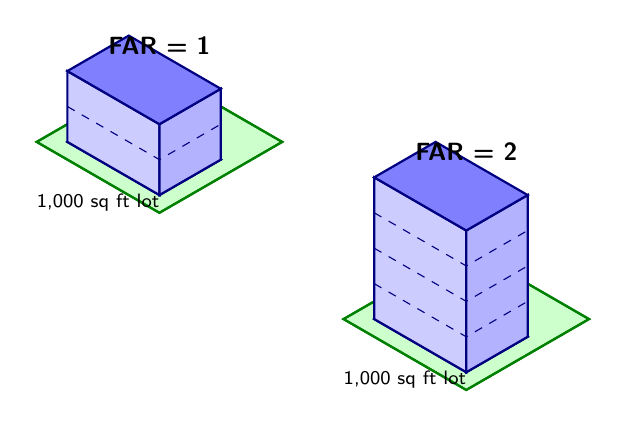
\begin{tikzpicture}[
            scale=0.45,
            x={(0.866cm,-0.5cm)},
            y={(0.866cm,0.5cm)},
            z={(0cm,1cm)},
            lot/.style={fill=green!20, draw=green!50!black, thick},
            building/.style={fill=blue!30, draw=blue!50!black, thick},
            building top/.style={fill=blue!50, draw=blue!50!black, thick},
            building side/.style={fill=blue!20, draw=blue!50!black, thick},
        ]
        % LEFT: FAR = 1
        \begin{scope}[shift={(-5,0,0)}]
            \fill[lot] (0,0,0) -- (4,0,0) -- (4,4,0) -- (0,4,0) -- cycle;
            \draw[green!50!black, thick] (0,0,0) -- (4,0,0) -- (4,4,0) -- (0,4,0) -- cycle;
            \def\bx{0.5} \def\by{0.5} \def\bw{3} \def\bd{2} \def\bh{2}
            \fill[building] (\bx,\by,0) -- (\bx+\bw,\by,0) -- (\bx+\bw,\by+\bd,0) -- (\bx,\by+\bd,0) -- cycle;
            \fill[building side] (\bx,\by,0) -- (\bx+\bw,\by,0) -- (\bx+\bw,\by,\bh) -- (\bx,\by,\bh) -- cycle;
            \fill[building] (\bx+\bw,\by,0) -- (\bx+\bw,\by+\bd,0) -- (\bx+\bw,\by+\bd,\bh) -- (\bx+\bw,\by,\bh) -- cycle;
            \fill[building top] (\bx,\by,\bh) -- (\bx+\bw,\by,\bh) -- (\bx+\bw,\by+\bd,\bh) -- (\bx,\by+\bd,\bh) -- cycle;
            \draw[blue!50!black, dashed] (\bx,\by,1) -- (\bx+\bw,\by,1) -- (\bx+\bw,\by+\bd,1);
            \node[font=\scriptsize\sffamily, below] at (2,0,-0.2) {1,000 sq ft lot};
            \node[font=\small\sffamily\bfseries, above] at (2,2,\bh+0.2) {FAR = 1};
        \end{scope}
        % RIGHT: FAR = 2
        \begin{scope}[shift={(5,0,0)}]
            \fill[lot] (0,0,0) -- (4,0,0) -- (4,4,0) -- (0,4,0) -- cycle;
            \draw[green!50!black, thick] (0,0,0) -- (4,0,0) -- (4,4,0) -- (0,4,0) -- cycle;
            \def\bx{0.5} \def\by{0.5} \def\bw{3} \def\bd{2} \def\bh{4}
            \fill[building] (\bx,\by,0) -- (\bx+\bw,\by,0) -- (\bx+\bw,\by+\bd,0) -- (\bx,\by+\bd,0) -- cycle;
            \fill[building side] (\bx,\by,0) -- (\bx+\bw,\by,0) -- (\bx+\bw,\by,\bh) -- (\bx,\by,\bh) -- cycle;
            \fill[building] (\bx+\bw,\by,0) -- (\bx+\bw,\by+\bd,0) -- (\bx+\bw,\by+\bd,\bh) -- (\bx+\bw,\by,\bh) -- cycle;
            \fill[building top] (\bx,\by,\bh) -- (\bx+\bw,\by,\bh) -- (\bx+\bw,\by+\bd,\bh) -- (\bx,\by+\bd,\bh) -- cycle;
            \foreach \h in {1,2,3} {
                \draw[blue!50!black, dashed] (\bx,\by,\h) -- (\bx+\bw,\by,\h) -- (\bx+\bw,\by+\bd,\h);
            }
            \node[font=\scriptsize\sffamily, below] at (2,0,-0.2) {1,000 sq ft lot};
            \node[font=\small\sffamily\bfseries, above] at (2,2,\bh+0.2) {FAR = 2};
        \end{scope}
        \end{tikzpicture}
        
        \vspace{0.5em}
        {\small $\text{FAR} = \dfrac{\text{Total Building Floor Area}}{\text{Lot Area}}$}
    \end{column}
    
    \begin{column}{0.43\textwidth}
        \small
        \textbf{FAR limits development intensity}
        
        \vspace{0.5em}
        Same lot, different allowed density:
        \begin{itemize}
            \item FAR = 1: Can build 1,000 sq ft
            \item FAR = 2: Can build 2,000 sq ft
        \end{itemize}
        
        \vspace{0.5em}
        \textbf{Chicago zoning examples:}
        \vspace{-0.3em}
        \begin{center}
        \scriptsize
        \begin{tabular}{lcc}
        \toprule
        Zone & Max FAR & Typical Use \\
        \midrule
        RS-3 & 0.9 & Single-family \\
        RT-4 & 1.2 & Two-flat \\
        RM-5 & 2.0 & Small apartment \\
        RM-6 & 4.4 & Mid-rise \\
        \bottomrule
        \end{tabular}
        \end{center}
    \end{column}
    \end{columns}
\end{frame}


% ==============================================================================
% SLIDE 13: WHAT IS DUPAC?
% ==============================================================================
\begin{frame}
    \frametitle{Density Outcomes: Dwelling Units Per Acre (DUPAC)}
    
    \begin{columns}[T]
    \begin{column}{0.55\textwidth}
        \centering
        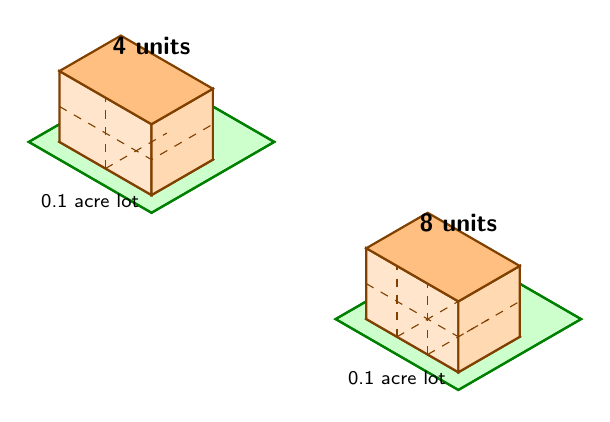
\begin{tikzpicture}[
            scale=0.45,
            x={(0.866cm,-0.5cm)},
            y={(0.866cm,0.5cm)},
            z={(0cm,1cm)},
            lot/.style={fill=green!20, draw=green!50!black, thick},
            building/.style={fill=orange!30, draw=orange!50!black, thick},
            building top/.style={fill=orange!50, draw=orange!50!black, thick},
            building side/.style={fill=orange!20, draw=orange!50!black, thick},
            unit/.style={fill=red!40, draw=red!60!black, thick},
        ]
        % LEFT: 4 units
        \begin{scope}[shift={(-5,0,0)}]
            \fill[lot] (0,0,0) -- (4,0,0) -- (4,4,0) -- (0,4,0) -- cycle;
            \draw[green!50!black, thick] (0,0,0) -- (4,0,0) -- (4,4,0) -- (0,4,0) -- cycle;
            \def\bx{0.5} \def\by{0.5} \def\bw{3} \def\bd{2} \def\bh{2}
            \fill[building] (\bx,\by,0) -- (\bx+\bw,\by,0) -- (\bx+\bw,\by+\bd,0) -- (\bx,\by+\bd,0) -- cycle;
            \fill[building side] (\bx,\by,0) -- (\bx+\bw,\by,0) -- (\bx+\bw,\by,\bh) -- (\bx,\by,\bh) -- cycle;
            \fill[building] (\bx+\bw,\by,0) -- (\bx+\bw,\by+\bd,0) -- (\bx+\bw,\by+\bd,\bh) -- (\bx+\bw,\by,\bh) -- cycle;
            \fill[building top] (\bx,\by,\bh) -- (\bx+\bw,\by,\bh) -- (\bx+\bw,\by+\bd,\bh) -- (\bx,\by+\bd,\bh) -- cycle;
            % Unit dividers
            \draw[orange!50!black, dashed] (\bx,\by,1) -- (\bx+\bw,\by,1) -- (\bx+\bw,\by+\bd,1);
            \draw[orange!50!black, dashed] (\bx+1.5,\by,0) -- (\bx+1.5,\by,\bh);
            \draw[orange!50!black, dashed] (\bx+1.5,\by,0) -- (\bx+1.5,\by+\bd,0);
            \node[font=\scriptsize\sffamily, below] at (2,0,-0.2) {0.1 acre lot};
            \node[font=\small\sffamily\bfseries, above] at (2,2,\bh+0.2) {4 units};
        \end{scope}
        % RIGHT: 8 units (same FAR, more units)
        \begin{scope}[shift={(5,0,0)}]
            \fill[lot] (0,0,0) -- (4,0,0) -- (4,4,0) -- (0,4,0) -- cycle;
            \draw[green!50!black, thick] (0,0,0) -- (4,0,0) -- (4,4,0) -- (0,4,0) -- cycle;
            \def\bx{0.5} \def\by{0.5} \def\bw{3} \def\bd{2} \def\bh{2}
            \fill[building] (\bx,\by,0) -- (\bx+\bw,\by,0) -- (\bx+\bw,\by+\bd,0) -- (\bx,\by+\bd,0) -- cycle;
            \fill[building side] (\bx,\by,0) -- (\bx+\bw,\by,0) -- (\bx+\bw,\by,\bh) -- (\bx,\by,\bh) -- cycle;
            \fill[building] (\bx+\bw,\by,0) -- (\bx+\bw,\by+\bd,0) -- (\bx+\bw,\by+\bd,\bh) -- (\bx+\bw,\by,\bh) -- cycle;
            \fill[building top] (\bx,\by,\bh) -- (\bx+\bw,\by,\bh) -- (\bx+\bw,\by+\bd,\bh) -- (\bx,\by+\bd,\bh) -- cycle;
            % More unit dividers (8 units)
            \draw[orange!50!black, dashed] (\bx,\by,1) -- (\bx+\bw,\by,1) -- (\bx+\bw,\by+\bd,1);
            \draw[orange!50!black, dashed] (\bx+1,\by,0) -- (\bx+1,\by,\bh);
            \draw[orange!50!black, dashed] (\bx+2,\by,0) -- (\bx+2,\by,\bh);
            \draw[orange!50!black, dashed] (\bx+1,\by,0) -- (\bx+1,\by+\bd,0);
            \draw[orange!50!black, dashed] (\bx+2,\by,0) -- (\bx+2,\by+\bd,0);
            \node[font=\scriptsize\sffamily, below] at (2,0,-0.2) {0.1 acre lot};
            \node[font=\small\sffamily\bfseries, above] at (2,2,\bh+0.2) {8 units};
        \end{scope}
        \end{tikzpicture}
        
        \vspace{0.5em}
        {\small DUPAC: 40 vs.\ 80 units/acre  (same building volume!)}
    \end{column}
    
    \begin{column}{0.43\textwidth}
        \small
        \textbf{DUPAC captures population density}
        
        \vspace{0.5em}
        $\text{DUPAC} = \dfrac{\text{\# Dwelling Units}}{\text{Lot Acreage}}$
        
        \vspace{0.5em}
        \textbf{Why both measures?}
        \begin{itemize}
            \item Same FAR, different DUPAC
            \item \textbf{Developers} care about FAR (total rentable space)
            \item \textbf{Neighbors} care about DUPAC (congestion, parking, schools)
        \end{itemize}
    \end{column}
    \end{columns}
\end{frame}


% ==============================================================================
% SLIDE 14: DATA - NEW MULTIFAMILY CONSTRUCTION
% ==============================================================================
\begin{frame}
    \frametitle{Data: New Multifamily Construction}
    
    \begin{columns}[T]
    \begin{column}{0.55\textwidth}
    \textbf{Source}: Cook County Assessor parcel data, 2006-2025
    
    \vspace{0.5em}
    \textbf{Sample}: Multifamily buildings with 2--100 units
    \begin{itemize}
        \item \textbf{Single family}: Majority of construction but less variation in density
        \item \textbf{Large developments} (100+ units): Planned Development process with more city oversight
    \end{itemize}
    
    \vspace{0.5em}
    \textbf{Why multifamily matters}: 
    \begin{itemize}
        \item Only $\sim$19\% of new construction but a dispraportionate share of total housing supply
    \end{itemize}
    \end{column}
    
    \begin{column}{0.43\textwidth}
    \textbf{Summary statistics}:
    \vspace{0.3em}
    \small
    \begin{tabular}{lcc}
    \toprule
     & All & MF Only \\
    \midrule
    Avg FAR & 1.22 & 2.32 \\
    Avg Units & 6.65 & 31.3 \\
    Avg Stories & 2.27 & 2.75 \\
    Avg DUPAC & 28.5 & 74.5 \\
    \midrule
    N & 13,236 & 2,469 \\
    \bottomrule
    \end{tabular}
    \end{column}
    \end{columns}
\end{frame}


% ==============================================================================
% SLIDE 15: IDENTIFICATION STRATEGY
% ==============================================================================
\begin{frame}
    \frametitle{Identification Strategy: Border Discontinuity}
    
    \textbf{Idea}: Compare new multifamily construction on opposite sides of ward boundaries
    \begin{itemize}
        \item Focus on parcels \textbf{within 500 feet} of border 
        \item Use stringent border-pair $\times$ year FEs to remove unobserved heterogeneity
    \end{itemize}
    
    \vspace{0.3em}
    \textbf{Identifying variation}: At the same border in the same year, does the stricter side have less dense construction?
    
    \vspace{0.3em}
    Two specifications:
    \begin{itemize}
        \item \textbf{Visual RD}: Descriptive, visual evidence of discontinuities at ward borders
        \item \textbf{Regressions}: Regression with continuous strictness measure and stringent FEs
    \end{itemize}
\end{frame}


% ==============================================================================
% SLIDE 16: VISUAL RD RESULTS
% ==============================================================================
\begin{frame}[label=visual-rd-main]
    \frametitle{Visual Evidence: Density Discontinuity at Ward Borders}
    
    \begin{columns}[T]
    \begin{column}{0.48\textwidth}
        \centering
        \textbf{Log(FAR)}
        \begin{figure}
            \includegraphics[width=\textwidth,height=0.55\textheight,keepaspectratio]{../tasks/spatial_rd_same_zone_only/output/rd_plot_log_density_far_bw500_triangular.pdf}
        \end{figure}
    \end{column}
    \begin{column}{0.48\textwidth}
        \centering
        \textbf{Log(DUPAC)}
        \begin{figure}
            \includegraphics[width=\textwidth,height=0.55\textheight,keepaspectratio]{../tasks/spatial_rd_same_zone_only/output/rd_plot_log_density_dupac_bw500_triangular.pdf}
        \end{figure}
    \end{column}
    \end{columns}
    
    \scriptsize
    \textit{Notes}: Stacked borders; lenient (left) vs.\ strict (right). 500 ft bandwidth.
    
    \vfill\hfill
    \hyperlink{visual-rd-placebo}{\beamergotobutton{Placebo Boundaries}}
    \hspace{0.2em}
    \hyperlink{visual-rd-functional}{\beamergotobutton{Functional Form}}
    \hspace{0.2em}
    \hyperlink{visual-rd-donut}{\beamergotobutton{Donut}}
\end{frame}


% ==============================================================================
% SLIDE 17: BORDER-PAIR FE RESULTS
% ==============================================================================
\begin{frame}[label=density-reg-main]
    \frametitle{Main Results: Border-Pair Fixed Effects}
    
    \small
    \textbf{Specification}: 
    $\ln(Y_i) = \beta \cdot \text{Strictness}_i + \alpha_{\text{border} \times \text{year} } + \varepsilon_i$\\
    Sample: Within 500 ft, 2-100 units. Standard errors clustered at border-pair level.
    
    \begin{center}
    \input{../tasks/border_pair_FE_regressions/output/fe_table_bw500_pair_x_year.tex}
    \end{center}
    
    \vspace{0.1em}
    \textbf{Interpretation}: A 1 SD $\uparrow$ in strictness $\rightarrow$ 13-15\% less dense multifamily construction
    
    \vspace{-0.4em}
    \vfill\hfill
    \hyperlink{density-reg-bw250}{\beamergotobutton{250ft}}
    \hspace{0.1em}
    \hyperlink{density-reg-bw1000}{\beamergotobutton{1000ft}}

\end{frame}


% PART 6: PRICE & RENT ANALYSIS (Slides 19-24)
% ==============================================================================
% EVENT STUDY SECTION
% Slides: From supply to prices, ID strategy, Data, Results
% ==============================================================================

% ==============================================================================
% SLIDE: FROM SUPPLY TO PRICES
% ==============================================================================
\begin{frame}
    \frametitle{From Density to Prices}
    
    \textbf{So far}: Stricter aldermen $\rightarrow$ lower multifamily density
    
    \vspace{0.5em}
    \textbf{Next question}: Does restricted supply affect housing costs?
    
    \vspace{0.5em}
    Exploit redistricting as natural experiment
    \begin{itemize}
        \item Ward boundaries redrawn after each decennial census (2015, 2023)
        \item Some census blocks reassigned to a new alderman while neighboring blocks do not
        \item Compare prices before vs.\ after reassignment
    \end{itemize}
\end{frame}


% ==============================================================================
% SLIDE: EVENT STUDY DESIGN
% ==============================================================================
\begin{frame}
    \frametitle{Event Study Design}
    
    \textbf{Intuition}: When a block switches from lenient $\rightarrow$ strict alderman, \\
    \hspace{4em} expected future supply $\downarrow$ $\Rightarrow$ prices should $\uparrow$
    
    \vspace{0.5em}
    \textbf{Specification}:
    \[
    \ln(P_{it}) = \sum_{\tau \neq -1} \beta_\tau \cdot \mathbf{1}[t = \tau] \cdot \Delta\text{Strictness}_i + X_{it}'\gamma + \alpha_{ps} + \lambda_{pt} + \varepsilon_{it}
    \]
    
    \vspace{-0.3em}
    \begin{itemize}
        \item $\Delta\text{Strictness}_i = \text{Strictness}_{\text{dest}} - \text{Strictness}_{\text{origin}}$ 
        \item $X_{it}$: Hedonic controls (sqft, beds, baths, building type/age)
        \item $\alpha_{ps}$: Border-pair $\times$ origin-side FE
        \item $\lambda_{pt}$: Border-pair $\times$ year FE
    \end{itemize}
    
    \vspace{0.5em}
    \textbf{Key assumption}: Parallel trends within each border-pair $\times$ side cell
    
    \vspace{0.3em}
    \small
    Sample: Within 1,000 ft of boundaries; triangular weights $w_i = 1 - \frac{d_i}{1000}$; SEs clustered by block
\end{frame}


% ==============================================================================
% SLIDE: IDENTIFICATION EXAMPLE
% ==============================================================================
\begin{frame}
    \frametitle{Identification: Example from Wards 13 \& 23}
    
    \begin{figure}
        \centering
        \includegraphics[width=1.1\textwidth,height=0.70\textheight,keepaspectratio]{../tasks/event_study_sales_diagnostics/output/ward_pair_before_after_13-23.pdf}
    \end{figure}
    
    \vspace{-0.5em}
    \small
    Blocks reassigned between wards with different strictness scores provide identifying variation.
    \hfill
    \hyperlink{treatment-maps}{\beamergotobutton{Citywide Maps}}
\end{frame}


% ==============================================================================
% SLIDE: EVENT STUDY DATA
% ==============================================================================
\begin{frame}[label=event-data]
    \frametitle{Event Study Data}
    
    \begin{columns}[T]
    \begin{column}{0.48\textwidth}
    \textbf{Rental Listings}
    \begin{itemize}
        \item Scraped rental listings from Renthub, 2014-2025
        \item Asking rents
        \item \textbf{Stacked design}: 2015 + 2023 cohorts (implementation date)
        \item N $\approx$ 3.9 million near borders
    \end{itemize}
    \end{column}
    
    \begin{column}{0.48\textwidth}
    \textbf{Home Sales}
    \begin{itemize}
        \item Cook County Assessor Data from Illinois Department of Revenue, 2007-2025
        \item Arms-length transactions only
        \item \textbf{Stacked design}: 2012 + 2022 cohorts (announcement date)
        \item N $\approx$ 78,000 near borders
    \end{itemize}
    \end{column}
    \end{columns}
    
    \vspace{0.5em}
    \textbf{Sample}: Transactions/listings within 1,000 ft of ward boundaries
    
    \vfill\hfill
    \hyperlink{treatment-details}{\beamergotobutton{Full Treatment \& Control Details}}
\end{frame}


% ==============================================================================
% SLIDE: RENT RESULTS - CONTINUOUS AND BINARY
% ==============================================================================
\begin{frame}[label=rent-main]
    \frametitle{Effect on Log(Rents)}
    
    \begin{columns}[T]
    \begin{column}{0.48\textwidth}
        \centering
        \textbf{Aggregate Treatment Effect}
        \begin{figure}
            \includegraphics[width=\textwidth,height=0.55\textheight,keepaspectratio]{../tasks/run_event_study_rental_disaggregate/output/event_study_disaggregate_yearly_stacked_continuous_triangular_1000ft_short.pdf}
        \end{figure}
    \end{column}
    \begin{column}{0.48\textwidth}
        \centering
        \textbf{Stricter vs. Lenient}
        \begin{figure}
            \includegraphics[width=\textwidth,height=0.55\textheight,keepaspectratio]{../tasks/run_event_study_rental_disaggregate/output/event_study_disaggregate_yearly_stacked_continuous_split_triangular_1000ft_short.pdf}
        \end{figure}
    \end{column}
    \end{columns}
    
    \vspace{0.2em}
    \small
    5\% rent increase two years after implementation \\
    Binary split confirms: stricter $\rightarrow$ rents rise; lenient $\rightarrow$ rents fall.
    
    \vfill\hfill
    \hyperlink{rent-bw500}{\beamergotobutton{500ft}}
    \hspace{0.2em}
    \hyperlink{rent-no-hedonics}{\beamergotobutton{No Controls}}
\end{frame}


% ==============================================================================
% SLIDE: HOME PRICE RESULTS - CONTINUOUS AND BINARY
% ==============================================================================
\begin{frame}[label=price-main]
    \frametitle{Effect on Log(Home Prices)}
    
    \begin{columns}[T]
    \begin{column}{0.48\textwidth}
        \centering
        \textbf{Aggregate Treatment Effect}
        \begin{figure}
            \includegraphics[width=\textwidth,height=0.55\textheight,keepaspectratio]{../tasks/run_event_study_sales_disaggregate/output/event_study_disaggregate_yearly_stacked_announcement_continuous_triangular_1000ft.pdf}
        \end{figure}
    \end{column}
    \begin{column}{0.48\textwidth}
        \centering
        \textbf{Stricter vs. Lenient}
        \begin{figure}
            \includegraphics[width=\textwidth,height=0.55\textheight,keepaspectratio]{../tasks/run_event_study_sales_disaggregate/output/event_study_disaggregate_yearly_stacked_announcement_continuous_split_triangular_1000ft.pdf}
        \end{figure}
    \end{column}
    \end{columns}
    
    \vspace{0.2em}
    \small
    Home prices show consistent but more muted patterns: $\sim$2\% increase five years after announcement \\
    
    \vfill\hfill
    \hyperlink{price-no-hedonics}{\beamergotobutton{No Controls}}
    \hspace{0.2em}
    \hyperlink{price-balance}{\beamergotobutton{Covariate Balance}}
\end{frame}


% ==============================================================================
% SLIDE: EVENT STUDY RESULTS - MAGNITUDES (DiD Tables)
% ==============================================================================
\begin{frame}
    \frametitle{Difference-in-Differences Estimates}
    
    \begin{columns}[T]
    \begin{column}{0.48\textwidth}
    \centering
    \textbf{Log(Rents)}
    \scriptsize
    \input{../tasks/run_event_study_rental_disaggregate/output/did_table_rental_clean.tex}
    \normalsize
    
    \vspace{0.5em}
    $\Rightarrow$ 1 SD $\uparrow$ strictness \\
    $\approx$ 3-5\% $\uparrow$ in rents
    \end{column}
    
    \begin{column}{0.48\textwidth}
    \centering
    \textbf{Log(Home Prices)}
    \scriptsize
    \input{../tasks/run_event_study_sales_disaggregate/output/did_table_sales_clean.tex}
    \normalsize
    
    \vspace{0.5em}
    $\Rightarrow$ 1 SD $\uparrow$ strictness \\
    $\approx$ 1.3\% $\uparrow$ in prices
    \end{column}
    \end{columns}
    
    \vspace{0.5em}
    \small
    Border-pair $\times$ side FE and border-pair $\times$ year FE. Triangular kernel, 1000 ft bandwidth.
    
    \hfill \hyperlink{price-balance}{\beamergotobutton{Covariate Balance}}
\end{frame}


% PART 7: CONCLUSION (Slides 25-26)
\section{Conclusion}
\label{sec:conclusion}

This paper examines how the fragmentation of land use authority within cities affects housing supply and prices. I study Chicago's ``aldermanic privilege'': the informal institution granting each of the city's 50 aldermen effective veto power over development in their ward—and document its consequences for housing markets.

I construct aldermanic strictness scores from permit processing times, using a residualization approach that removes the influence of ward characteristics and an empirical Bayes procedure that addresses measurement error for aldermen with few permits. The resulting scores reveal substantial and persistent variation in regulatory stringency across aldermen that is not simply a reflection of geography or neighborhood demographics.

Using these scores, I employ two complementary empirical strategies. First, a spatial discontinuity design comparing development density on opposite sides of ward boundaries finds that new construction is 10-16\% less dense on the stricter side of ward boundaries, with effects concentrated within 250 feet of the boundary. Second, event studies exploiting the 2012 announcement and 2015 implementation of ward redistricting show that home prices rise approximately 4\% when census blocks are reassigned to stricter aldermen, with effects beginning at announcement—suggesting that housing markets are forward-looking with respect to regulatory changes. Rents rise 3-5\% following reassignment to stricter aldermen, though these estimates are less precise.

These findings have several implications. First, within-city fragmentation of land use authority can generate coordination failures analogous to those documented across municipalities: individual decision-makers rationally restrict development, but the collective outcome is undersupply of housing relative to the social optimum. Second, the effects of regulatory stringency are highly localized—concentrated near ward boundaries where the jurisdiction of strict and lenient aldermen meet—suggesting that developers are attentive to aldermanic preferences at fine spatial scales. Third, housing markets capitalize expected future regulation, not just current policy, implying that credible reforms to aldermanic privilege could affect prices even before implementation.

Several limitations warrant mention. The estimates presented here do not capture the extensive margin ``deterrence'' effects and likely represent lower bounds of the true impact, as the considered projects that are never proposed are unobserved. The analysis focuses on local, partial-equilibrium effects and does not capture citywide general-equilibrium adjustments to changes in aldermanic strictness. And while the event study design supports causal interpretation, I cannot fully separate supply-side mechanisms (aldermen restricting construction) from demand-side mechanisms (stricter aldermen signaling neighborhood desirability) in explaining price effects.

Future work could extend this analysis in several directions: quantifying the welfare costs of aldermanic privilege using a structural model of developer and household location choice; examining whether aldermanic strictness affects the composition of housing supply, particularly affordable versus market-rate units; and studying whether electoral competition or transparency requirements discipline restrictive behavior. Extending the empirical approach to other cities with ward-based governance could assess the external validity of these findings.

Chicago's ongoing debate over aldermanic privilege is not merely symbolic. The institution has real, quantifiable effects on where housing gets built and how much it costs. As cities across the United States grapple with housing affordability crises, understanding how local political institutions shape housing supply is essential. The evidence presented here suggests that reforming fragmented land use authority through some combination of centralization, by-right development, or other mechanisms could meaningfully improve housing market outcomes.


%---------------------------------------------------------------------
\begin{frame}[plain]
    \begin{center}{\LARGE Thank you!}\end{center}
\end{frame}
%---------------------------------------------------------------------

%---------------------------------------------------------------------
% A frame to display the bibliography
\begin{frame}[allowframebreaks]{}
    \bibliographystyle{aer}
    \bibliography{sections/aldermanic_privilege}
\end{frame}
%---------------------------------------------------------------------

%---------------------------------------------------------------------
% Start appendix section
\appendix
%---------------------------------------------------------------------

%---------------------------------------------------------------------
% BACKUP SLIDES: Density Robustness
%---------------------------------------------------------------------
\begin{frame}[label=density-robustness]
    \frametitle{Robustness: Bandwidth Sensitivity}
    \begin{center}
    \textit{[Insert bandwidth sensitivity figure here]}
    \end{center}
    
    \vspace{1em}
    Effects stable across 250 ft, 500 ft, 1000 ft bandwidths.
    
    \vfill\hfill
    \hyperlink{density-donut}{\beamergotobutton{Donut RD}}
    \hspace{0.2em}
    \hyperlink{density-functional}{\beamergotobutton{Functional Form}}
    \hspace{0.2em}
    \hyperlink{density-balance}{\beamergotobutton{Covariate Balance}}
\end{frame}

\begin{frame}[label=density-donut]
    \frametitle{Robustness: Donut RD}
    \begin{center}
    \textit{[Insert donut RD figure here]}
    \end{center}
    
    \vspace{1em}
    Excluding parcels within 25--50 ft of border does not change results.
\end{frame}

\begin{frame}[label=density-functional]
    \frametitle{Robustness: Functional Form}
    \begin{center}
    \textit{[Insert functional form comparison here]}
    \end{center}
    
    \vspace{1em}
    Results robust to linear, quadratic, and cubic polynomial specifications.
\end{frame}

\begin{frame}[label=density-balance]
    \frametitle{Covariate Balance at Ward Borders}
    \begin{center}
    \textit{[Insert balance table here]}
    \end{center}
    
    \vspace{1em}
    Demographics smooth across ward boundaries.
\end{frame}

%---------------------------------------------------------------------
% BACKUP SLIDES: Price/Rent Robustness
%---------------------------------------------------------------------
\begin{frame}[label=price-robustness]
    \frametitle{Robustness: Pre-Trends and Placebo Tests}
    \begin{center}
    \includegraphics[width=0.8\textwidth,height=0.6\textheight,keepaspectratio]{../tasks/event_study_sales_diagnostics/output/pre_trend_coefficients.pdf}
    \end{center}
    
    \vspace{0.5em}
    Joint test of pre-period coefficients: Cannot reject null of zero pre-trends.
\end{frame}

\begin{frame}[label=price-hedonics]
    \frametitle{Robustness: With and Without Hedonic Controls}
    \begin{center}
    \textit{[Results stable with/without hedonic controls --- see main tables]}
    \end{center}
    
    \vspace{1em}
    Adding building characteristics (sqft, age, bedrooms, bathrooms, garage) does not substantially change point estimates.
\end{frame}


\end{document}
